\documentclass[a4paper,12pt]{article}
\usepackage[T1]{fontenc}
\usepackage[utf8]{inputenc}
\usepackage[english]{babel}
\usepackage[a4paper,margin=2.5cm]{geometry}

% Math, graphics, and nicer tables
\usepackage{amsmath,amssymb, amsfonts}
% Number equations within sections (gives (1.1), (1.2), ...)
\numberwithin{equation}{section}
\usepackage{graphicx}
\usepackage{booktabs}
\usepackage{caption}
\usepackage{subcaption}
\usepackage{enumitem}
\usepackage{asymptote}
\usepackage{listings}
\usepackage{xcolor}

\lstdefinestyle{cpp}{
    language=C++,
    basicstyle=\ttfamily\small,
    numbers=left,
    numberstyle=\tiny,
    keywordstyle=\color{blue},
    commentstyle=\color{green!50!black},
    stringstyle=\color{red},
    frame=single,
    breaklines=true,
    tabsize=4
}

% Bibliography and hyperlinks

\usepackage{caption}
\usepackage{subcaption}

% Bibliography and hyperlinks
\usepackage[english]{babel}
\usepackage[square,numbers]{natbib}
\usepackage[unicode=true,bookmarks=true,colorlinks=true,linkcolor=blue,citecolor=red,backref=page]{hyperref}
\usepackage{cleveref}

% Example placeholder images (from package 'mwe') if available; otherwise replace with your image files
\usepackage{mwe} % provides example-image

\title{\textbf{Numerical Methods for Non-Linear Mechanics}}
\author{Viet Anh Quach}


\begin{document}
\maketitle


% \begin{abstract}

% \end{abstract}

\section{Introduction}
This short report present the code that is assign for the subject "Numerical Methods for Non-Linear Mechanics" of the Master Program for Civil Engineering, teached by professor Stafano-Dal Pont at Laboratory 3SR, University Grenoble Alpes, France.
The object of the course is studying the non-linear problems in mechanics, caused by both the geometric and material behavior.
The assigment practices therefore is to build in the most general form of the constitutive law, which is not linearity.
2 main problems are takin into account: A console problem in 2D and a Truss problem in 3D, hence the remaining of this reports are divided into two sections of the former subject. 
Besides, this is a ideal chance to practice, thus I also try to provide a solution for the problem of Finite Element Method in 1D and 2D.
The main code is actually written in \texttt{C++}, with libraries mostly building from scratches. They have been upload to \texttt{Github}, the link to download is provided in \cref{Annexxe}. 
The plotting is realized by \texttt{Asymptote} - a vector graphic language with C-like features. The whole purpose is to learn so any corrections and comments are highly appreciated.
I would like to thank the professors for letting me, even though being a PhD student, could join this program to learn. I really appreciated and enjoyed the class.

\section{Theory}
The following problem was fully described in lecture course \citep{dalpont2020_nonlinear_mech} of professor \citeauthor{dalpont2020_nonlinear_mech}.
This section just represent it but with the particular methods using within the following codes and the reasons of these choice.

\subsection{Console}

\begin{figure}[h]
  \centering
  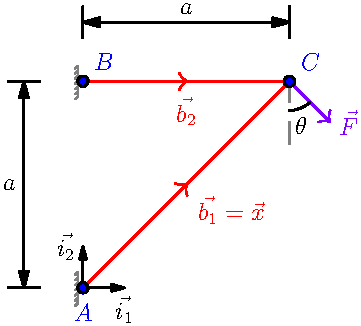
\includegraphics[height=5cm]{console2D.pdf}
  \caption{Two elements truss: console 2D}
  \label{truss2D}
\end{figure}
We begin with the most simplified problem which the whole geometry is described in \cref{truss2D}.
Briefly speaking, the simple truss structure is in 2 dimensions, composed by 3 nodes linked by 2 bars only. External force $F$ applied on the node $C$ maing an angel $\theta$ with the vertical axis, causing the displacement of the bars and nodes. Gravity is not taken into account.
In this case, $\vec{x}$ representing position of node $C$ is considered as the main unknown, owing to the fact that it is the only free node and fully represent the equilibrium position of the system.
 $\hat{e}^b$ is the unit vector of the corresponding bar $b$, which is calculated by the position vector of the node where the bar $b$ begins ($\vec{x}^B$) and ends ($\vec{x}^E$) :
 \begin{subequations}\label{eq:barVectors}
\begin{align}
  \vec{b} &= \vec{x}^{E(b)} - \vec{x}^{O(b)}\\
  l^{b} &= \|\vec{b}\|\\
  \hat{e}^b &= \dfrac{\vec{b}}{l^b} 
\end{align}
\end{subequations}
In truss elements, the only internal effort considered is the axial stress and further, also is a constant.
To satisfy the nodal equilibrium, at position $C$ the sum of the internal force (left-hand side) and the external force (right-hand side) must be balanced:
  \begin{equation}
     \sum_{b=1}^2  N^b =  N^1 + N^2 = F
  \label{consoleEquilibrium}
 \end{equation}
which $N^b$ denotes this component that the right part exerts on the left part of bar $b$, which is assumed to depend only on the length of bar $l^b$ via the constitutive law:
  \begin{equation}
     N^b = \mathcal{A}^b (l^b)
  \label{generalConstitutiveLaw}
 \end{equation}
In case of large displacement, this relation is no longer linear, as the bar's vectors are changed accordingly with the new position of the nodes, in our case is particularly node $C$.
The following elastic constitutive laws may be considered, so that the tension $N^b$ taken into account only on the bar length variation:
\begin{enumerate}[label=-]
  \item Linear law:   \begin{equation}
    \mathcal{A}^b (l^b) = \alpha^b \dfrac{l^b - l^b_0}{l^b_0}
    \label{linearLaw}
  \end{equation}
  \item Saint-Venant Kirchhoff law:
  \begin{equation}
    \mathcal{A}^b (l^b) = \alpha^b \dfrac{(l^b)^2 - (l^b_0)^2}{2 (l^b_0)^2}
    \label{kirchhoffLaw}
  \end{equation}
  \item Logarithmic law:
\begin{equation}
    \mathcal{A}^b (l^b) = \alpha^b ln(\dfrac{l^b}{l^b_0})
    \label{logarithmicLaw}
  \end{equation}
\end{enumerate}
Hence, in general form, the problem of the console could be written as follows:
  \begin{align}
    \text{Given the force } \vec{\mathcal{F}}, \nonumber\\
    \text{Find the position } \vec{x} \text{ of node C such that,} \nonumber\\
      -\mathcal{A}^1 (l^1(\vec{x})) \hat{e}^1(\vec{x}) -  \mathcal{A}^2 (l^2(\vec{x})) \hat{e}^2(\vec{x}) + \vec{\mathcal{F}} = \vec{0}
  \label{nodeEquilibrium2D}
 \end{align}

 This problem is solved by Newton's iterative method in vector form for solving systems of equations.
 For the order-one truncated Taylor series expansion, expression at the iteration (k+1) shall be:
  \begin{equation}
     \nabla \vec{\mathcal{F}} (\vec{x}^{(k)}) @ \delta (\vec{x}^{(k)}) = -\vec{\mathcal{{F}}}\left(\vec{x}^{(k)}\right)
  \label{NewtonMethod}
 \end{equation}
 Solving the linear system get us the new value of $\delta x$, so we could update the position for the next iteration by:
   \begin{equation}
 \vec{x}^{(k+1)} = \vec{x}^{(k)} + \delta \vec{x}^{(k)}
  \label{updatePosition}
 \end{equation}
 Apply to the console problem \cref{NewtonMethod} becomes 
 The method requires a stopping criterion: \cref{forceStop} is chosen to be implemented in the code, as it satisfies the force equilibrium condition at nodes of the problem.
 \begin{equation}
     \left| f\bigl(x^{(k)}\bigr) \right| < \epsilon
     \label{forceStop}
   \end{equation}
      where $\epsilon$ is a number small enough to be considered as 0, relatively to the problem solving.
   Another substitute approch is stopping at the iteration where the displacement is neglectable, which will be used in \cref{theoryTruss}:
    \begin{equation}
     \left| x^{k+1} - x^k \right| < \epsilon
     \label{displacementStop}
   \end{equation}
The object is now to transform equation \cref{generalConstitutiveLaw} into a linear form \cref{NewtonMethod} so that it could be numerically solved. 
Thanks to first-order Taylor expansion again, we obtain the development of sum of the force, which should be approching 0, at iteraion \texttt{k+1} (or in another word, at when node \textbf{C} would take an increment in position into $\vec{x}+ \delta \vec{x}$):
 \begin{equation}
  \vec{\mathcal{F}}(\vec{x}+ \delta \vec{x}) = \vec{\mathcal{F}}(\vec{x}) + \left(\nabla\vec{\mathcal{F}}(\vec{x})\right)@\delta \vec{x}  \rightarrow 0
  \label{TaylorK+1}
   \end{equation}
   where the Jacobian matrix $\nabla\vec{\mathcal{F}}(\vec{x})$ is described in the following euqation using Einsten's sum notation:
   \begin{equation}
   \nabla\vec{\mathcal{F}}(\vec{x}) = -\dfrac{d\mathcal{A}^i}{dl^i}\left( \vec{e}^i(\vec{x}) \otimes \vec{e}^i(\vec{x}) \right) - \dfrac{\mathcal{A}^i\left(l^i(\vec{x})\right)}{l^i(\vec{x})} \left( \mathbb{I} - \vec{e}^i(\vec{x}) \otimes \vec{e}^i(\vec{x})\right)
  \label{Jacobian}
   \end{equation} 
   Finally, we can solve the system using a single linear vector equation, which is suitable to be implemented into computational calculating:
    \begin{equation}
\left(\nabla\vec{\mathcal{F}}(\vec{x}^k)\right)@\delta \vec{x}^k =  - \vec{\mathcal{F}}(\vec{x}^k)
  \label{finalConsole}
   \end{equation}
   The first iteration starts from the initial condition of the system, then the iteration begins, until the residual $\vec{\mathcal{F}}(\vec{x}^k) < \epsilon$ could be considered null, as discussed above.

   \subsection{Truss} \label{theoryTruss}
\begin{figure}[h]
  \centering
  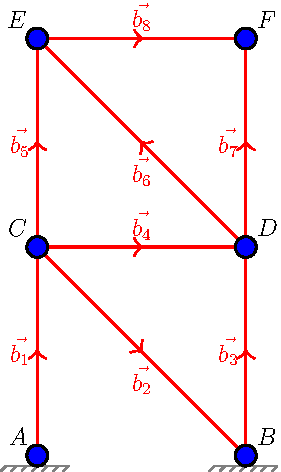
\includegraphics[height=6cm]{truss.pdf}
  \caption{3D truss}
  \label{truss3D}
\end{figure}
The 3D truss problem is a problem enhanced from the previous, which is in 3 dimensions and the numbers of bars could be as numerous as required.
Similarly in the previous problem, each bar's geometry is fully accessible through the position of nodes. Their vectors could be determined totally similar in the previous problem via \cref{eq:barVectors}.
The problem of the small deformation truss can be stated as:

  \begin{align}
    \text{Given the external force } \vec{F}^{e/n}, n \in \mathcal{N}_F \text{ and } \vec{U}^{n}, n \in \mathcal{N}_I \nonumber\\
    \text{find the displacement vector } \vec{u}^n, n \in \mathcal{N} \text{ so that } \vec{u}^n = \vec{U}^n, n \in \mathcal{N}_I \text{ and } \nonumber\\
      \forall\vec{v}^n \text{ such that } \vec{v}^n = 0, n \in \mathcal{N}_I \nonumber \\
      \sum_{b \in \mathcal{B}} k^b \vec{e}_0^b \left( \vec{u}^{E(b)} - \vec{u}^{O(b)}\right) \vec{e}_0^b \left( \vec{u}^{E(b)} - \vec{u}^{O(b)}\right) = \sum_{n \in \mathcal{N}_F} \vec{F}^{e/n} \vec{v}^n 
      \label{nodeEquilibrium3D}
 \end{align}
which expressed in matrix notation as:
   \begin{equation}
    \forall \underline{\mathcal{V}}^t \underline{\underline{\mathcal{K}}} \underline{\mathcal{U}} = \underline{\mathcal{V}}^t \underline{\mathcal{F}}  
   \end{equation} 
    or in the simpliest way:  
    \begin{equation}
 \underline{\underline{\mathcal{K}}} \ \underline{\mathcal{U}} = \underline{\mathcal{F}} \label{KU=F}
   \end{equation}
   We can easily verify that:
       \begin{equation} \underline{\mathcal{F}} = 
\begin{bmatrix}  
F_1^{e/1}\\
F_2^{e/1}\\
F_3^{e/1}\\
\vdots\\
F_1^{e/N}\\
F_2^{e/N}\\
F_3^{e/N}\\
\end{bmatrix}   ;\quad \underline{\mathcal{U}} = 
\begin{bmatrix}  
u_1^{1}\\
u_2^{1}\\
u_3^{1}\\
\vdots\\
u_1^{N}\\
u_2^{N}\\
u_3^{N}\\
\end{bmatrix}
\end{equation}
Within each component the subscript $k = 1,2,3$ stands for the 3 directions in 3D and the superscript $n = 1..N$ determines indices of nodes.

Meanwhile, the global stiffness matrix $\underline{\underline{\mathcal{K}}}$ could be assembled by multiple methods. One of them is by using the elementary application $K^b$ of bar $b$ along with the connectivity matrix $\underline{\underline{C^n}}$ as followed:

\begin{align}
  \underline{\underline{\mathcal{K}}} &= \sum_{b \in \mathcal{B}} \left( \underline{\underline{C}}^{E(b)} - \underline{\underline{C}}^{O(b)}\right) \underline{\underline{K}}^b \left( \underline{\underline{C}}^{E(b)} - \underline{\underline{C}}^{O(b)}\right) \\
  \underline{\underline{C^n}} & =
  \left[
  \begin{array}{@{}ccc|ccc|ccc@{}}
    0 & \cdots & 0 & 1 & 0 & 0 & 0 & \cdots & 0 \\
    \vdots & \ddots & \vdots & 0 & 1 & 0 & \vdots & \ddots & \vdots \\
    0 & \cdots & 0 & 0 & 0 & 1 & 0 & \cdots & 0
  \end{array}
  \right] \label{connectivityMatrix} \\
  &\qquad
  \begin{array}{@{}c@{\ }c@{\ }c@{}}
    \underbrace{\hspace{1.8cm}}_{3(n-1)} \ &
    \underbrace{\hspace{1.3cm}}_{3} \ &
    \underbrace{\hspace{1.8cm}}_{3(N-n)}
  \end{array}
\end{align}
Though this method is easily implemented in coding small problem, when calculating manually by hand, we prefer using the elementary stiffness matrix 
\begin{equation}
  \underline{\underline{\mathcal{K}}}^b = \underline{\underline{K}}^b 
  \begin{bmatrix}
    1 & -1 \\
    -1 & 1 
  \end{bmatrix} \label{elementaryStiffness}
\end{equation}
At this point, $\underline{\underline{\mathcal{K}}}$ should be singular i.e  $\det(\underline{\underline{\mathcal{K}}})=0$ because the kinematic boundary condition is not yet applied. Two different techniques are usually proposed: the direct method and the approximated method (so-called penalization method).
The approximated is obtained by adding $1/\epsilon$ to the main diagonal terms of $\underline{\underline{\mathcal{K}}}$ which corresponds to the nodes of $\mathcal{N}_I$:
   \begin{equation}
\underline{\underline{\mathcal{K}}}^{\epsilon}_{ii} = \underline{\underline{\mathcal{K}}}_{ii} + \dfrac{1}{\epsilon}; i = 3(n-1) + k; n \in \mathcal{N}_I, k = 1,2,3
\label{penalizationK}
\end{equation} 
% \subsection{Hardening}
\subsection{FEM1D}
\begin{figure}[h]
  \centering
  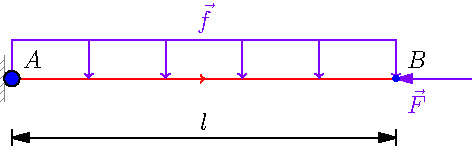
\includegraphics[height=2.5cm]{fem1D.pdf}
  \caption{1D Finite Element}
  \label{truss3D}
\end{figure}
The equilibrium equations therefore, described in the strong form:
\begin{subequations}
\begin{align}
  \dfrac{dN}{dx} + f &= 0;\\
  N(0) &= -R;\\
  N(l) &= F;\\
  N &= EA \dfrac{du}{dx};\\
  u(0) &= 0;
\end{align}
\end{subequations}
The weak form is expressed by;
\begin{equation}
   \forall v \in V, \int^l_0 EA \dfrac{du}{dx}\dfrac{dv}{dx}dx - Rv(0) = \int^l_0fvdx + Fv(l)
  \label{weakformFEM1D}
\end{equation}
\begin{equation}
  \forall v \in V, a(u,v) + b(R,v) = L(v)
  \label{weakformFEM1Dcompacted}
\end{equation}
rewritten in tensor notation:
\begin{align}
  \text{Find $\underline{\mathcal{U}}$ and $\mathcal{R}$ such that:}\\
 U^1 &= 0;\\
 \underline{\underline{\mathcal{K}}}\underline{\mathcal{U}} + \mathcal{R} &= \underline{\mathcal{F}}
  \label{FEM1D}
\end{align}
\subsection{FEM2D}
\begin{figure}[h]
  \centering
  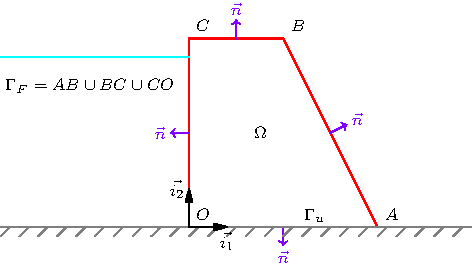
\includegraphics[height=6cm]{fem2D.pdf}
  \caption{Deformed console}
  \label{truss3D}
\end{figure}
\begin{align}
  \forall \vec{x} \in \Omega, \text{div} \sigma + \vec{f} &= 0;\\
  \forall \vec{x} \in \Omega,  \sigma &= \lambda \text{tr} \epsilon (\vec{u}) \mathbb{I} + 2\mu\epsilon(\vec{u});\\
    \forall \vec{x} \in \Gamma_u, \vec{u} &= \vec{U};\\
    \forall \vec{x} \in \Gamma_F, \sigma @\vec{n} &= \vec{F};\\
    \forall \vec{x} \in \Gamma_u, \sigma @\vec{n} &= \vec{R};\\
\end{align}
weak form:
\begin{align}
  \text{Find $\vec{u} \in V_0$ and $\vec{\mathcal{R}}$ such that:}\\
\forall \vec{v} \in V, \int_\Omega (\lambda \text{tr} \epsilon (\vec{u})\text{tr} \epsilon (\vec{v}) + 2\mu\epsilon(\vec{u}) : \epsilon(\vec{v}))ds - \int_{\Gamma_u}\vec{R}\vec{v}dl = \int_\Omega\vec{f}\vec{v}ds + \int_{\Gamma_F}\vec{F}\vec{v}dl;
  \label{FEM2D}
\end{align}
\section{Validation}
\subsection{Console}


Assume the bar to be rectangle, the input parameters are put in a namespace \texttt{modelParameters} within the code so one could change it accordingly to needs.
\begin{lstlisting}[style=cpp]
namespace modelParameters {
// Bar's parameters
double E{25e9}; // Module Young
double a{10.0}; // Distance between node 0 and 1 = bar length

double force{1.5e6};                // Imposed Force
// Inclined angle between the force with relative to vertical axis
double theta{20};

// Section dimension (rectangle)
double b1{0.02}, h1{0.05};
double b2{0.02}, h2{0.05};

// tolerance for Newton's method
double epsilon{1e-8};

// Choosing non-linear Saint-Venant Kirchhoff law
int law{1}; 
}
\end{lstlisting}

The final result obtained is:
\begin{verbatim}
=== 2D CONSOLE PROBLEM ===
Iteration 0: |Fk| = 1.5e+06: |dx| = 2.48569
Iteration 1: |Fk| = 814055: |dx| = 0.312942
Iteration 2: |Fk| = 19706.4: |dx| = 0.0172449
Iteration 3: |Fk| = 42.1839: |dx| = 3.20384e-05
Iteration 4: |Fk| = 0.00015477: |dx| = 1.26595e-10
Solution founded.

Final displacement: [0.526986, -2.14187]
Final position: [10.527, 7.85813]
Total iterations: 5
Time elapsed: 0.000276144 seconds
\end{verbatim}


\begin{figure}[h]
    \centering
    \begin{subfigure}[b]{0.48\textwidth}
        \centering
        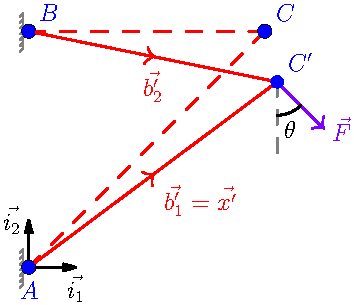
\includegraphics[height=5cm]{console2D_results.pdf}
        \caption{Deformed console schematic}
        \label{consoleDeformed}
    \end{subfigure}%
    \begin{subfigure}[b]{0.48\textwidth}
        \centering
        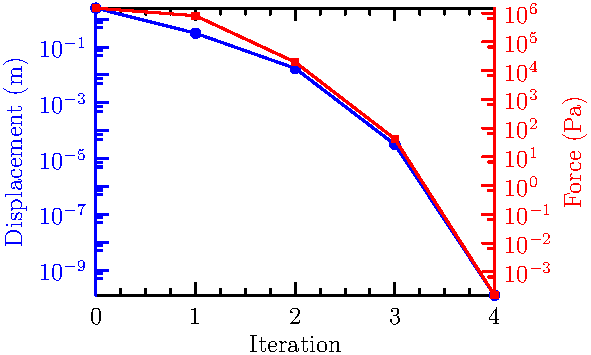
\includegraphics[height=5cm]{console_plot.pdf}
        \caption{Displacement and sum of forces on node C}
        \label{plotConsole}
    \end{subfigure}
    \caption{Solutions of the 2D console problem}
    \label{solutionFEM1D}
\end{figure}

As showed in diagram \cref{consoleDeformed}, under the effect of force $\vec{F}$, node C displaced from position (10,10) to (10.53, 7.86). These values are all justified by calculation manually and other codes.

As proved in figure \cref{plotConsole}, the rate of convergence (in logarithm proportion) by Newton method is quadratic.
Student choosed the Saint-Venant Kirchhoff law to present the result, with the intention to capture the non-linearity in both the constitutive law via \cref{generalConstitutiveLaw} and the large deformation's effect in \cref{eq:barVectors}.
\subsection{Truss}
\subsection{FEM1D}
Taking trivial value as follows: $f = 5kN;\ F = 10kN;\ EA = 10 kN;\ L = 1m$, once could verify the anylytic solution to be: $R = -15 kN; \ u(x) = 1.5x - 0.25x^2 (m);\ N(x) = 15 - 5x (kN);$
Using the script, though the reaction force at the first node $R (x=0) = -15$kN is always calculated precisely, the deformation $u(x)$ and the axial force $N(x)$ are highly depended on the number of nodes.
\Cref{solutionFEM1D} shows the numerical solution of the code, comparing with the analytical one. It was shown that the deformation $u(x)$ is obviously more precise, when the bar is discretized by using more elements.
The particular point of \texttt{FEM} comparing with Galerkin's method is using special shape function, particularly in this case is first-order hat function, via Lagrange's basis. This is well explained by when we discretized $u(x) = N_j u_j$. As $u_j$ is a constant, $u(x)$ is a first order polynomial (\cref{deformationFEM1D}), leading to its derivative to be a constant, hence $N(x) = EA\ du/dx $ is a constant on each element also (\cref{axialforceFEM1D}).

\begin{figure}[h]
    \centering
    \begin{subfigure}[b]{0.48\textwidth}
        \centering
        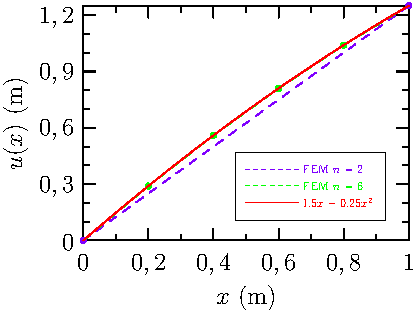
\includegraphics[height=6cm]{fem1D_u.pdf}
        \caption{Deformation}
        \label{deformationFEM1D}
    \end{subfigure}
    \hfill
    \begin{subfigure}[b]{0.48\textwidth}
        \centering
        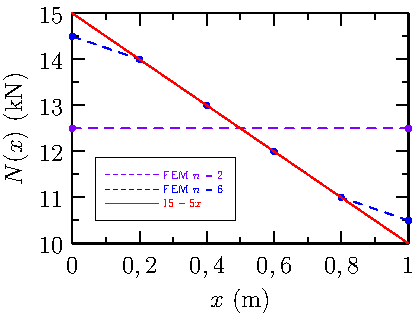
\includegraphics[height=6cm]{fem1D_N.pdf}
        \caption{Axial Force}
        \label{axialforceFEM1D}
    \end{subfigure}
    \caption{Solutions of the 1D FEM problem}
    \label{solutionFEM1D}
\end{figure}

\subsection{FEM2D}
In constructing...Stucking at the generation of the mesh.....
\section{Application Conclusion}
\subsection{Console}
The code is able to handle 2D Truss problems with 2 nodes, as a trial solution to the 3D truss problem following.
\subsection{Truss}
The code is able to handle any non-linear truss problem, 2D and 3D, including the console problem above. Though the Hardening incremented law should be implemented in the future to wider the range of problem that could be handled.
\subsection{FEM1D}
The code has been implemented in a way to solve any 1D bar problmem, with whatever the constraint conditions are, both Dirichlet and Neuman's condition. As long as the differential equation satisfied the form $u_{xx} = f(x) + c$ with $f(x)$ is a polynomial function of x, including $cx^0$.
This leads to the application of distributed load and concentration load exhibited on the bar.
Though the numerical cost could be reduced strongly using reference element, element Matrix, ... etc but this initial version is to test out all the functioning of the sub-coded also. Gladly, the solution seems to adapted well with the analytical one as expected.
\section{Conclusion}
In a nutshell, the code provided trustable result. Further implemented still rested to continue.
Thanks to using C++, time elapsed to execute one code is less then $10^{-3}$ second on the student's computer.
Further optimization...
\section[Annexxe]{Annexxe}\label{Annexxe}
Full version of the codes, including libraries used, could be downloaded in this \href{https://github.com/VA-TT/Numerical-Method-3SR}{link}.

\bibliographystyle{apalike}
\bibliography{Bibliography}

\end{document}